% XXX Jedes Jahr Mensa-Preise prüfen!
\section[Das kleine Mensa~1~×~1]{\boldmath Das kleine Mensa~${1 \times 1}$}
\begin{multicols*}{2}
\begin{quote}
	\textit{Allein zu essen ist für einen philosophierenden Gelehrten ungesund.}
	
	\hfill--- Immanuel Kant
\end{quote}

Alltäglich gegen Mittag beginnt der Magen zu knurren.
Für die Leute, die nicht jeden Tag nach Hause fahren oder selber kochen können -- also wenn Mutti zu weit weg wohnt -- gibt es die Mensa.
Das Gute ist, dass die Mensa~am~Ring direkt nebenan liegt.
Die meisten Studierenden gehen zwischen 11:45~Uhr und 12~Uhr direkt nach den Vorlesungen in die Mensa.

Dort erwartet euch dann meist eine große Schlange, denn um 12~Uhr ist der Anlauf dort am größten – die Chemiker halten Vorlesungen oft bis Punkt zwölf und kombinieren sich mit Trödlern und Leuten, die einen weiteren Weg haben. Ältere Semester (oder Leute die dies hier gelesen haben) werden sich daher entweder gegen 11:45~Uhr beeilen, oder wenn möglich ein wenig warten. Um etwa 12:20~Uhr ist es meist schon wieder wesentlich leerer.
Doch diese Schlange ist meist nach kurzer Zeit überwunden und da man normalerweise in Gruppen essen geht auch nicht so schlimm. Schwieriger ist da die Platzsuche, insbesondere für größere Gruppen. Gegen 12~Uhr ist die Mensa am vollsten, sodass vier Personen probleme kriegen können zusammen zu sitzen, danach lehrt sie sich langsam wieder. um etwa 12:20~Uhr wird man kaum noch Sitzplatzprobleme haben.
Bevor man sich anstellt, sollte man allerdings so einiges über die Mensa wissen!

Seit dem Sommersemester 2017 benötigt man zum Bezahlen lediglich seinen Studierendenausweis.
Das Guthaben darauf kann an den Automaten im Foyer der Mensa aufgeladen werden.
Wenn das Guthaben nicht mehr ausreicht um euer Essen zu bezahlen, könnt ihr den Ausweis auch an der Kasse noch aufladen. 
Das ist jedoch mit einem kleinen Aufpreis behaftet und die Missgunst der Kassiererin, sowie aller die in der Schlange hinter euch stehen ist euch sicher.
Falls ihr den Studierendenausweis noch nicht zugeschickt bekommen habt, könnte das daran liegen, dass ihr noch kein Foto dafür hochgeladen habt.
Das solltet ihr dann so bald wie möglich nachholen (textit{insbesondere weil ihr diesen auch als Bibliotheksausweis und für die Benutzung eures Semestertickets braucht}).

\begin{center}
	\includegraphics[width=\columnwidth]{private/res/studierendenausweis.pdf}
\end{center}

Viel wichtiger aber stellt sich jeden Mittag erneut die Frage, was es überhaupt zu Essen gibt und was du selbst essen willst.
Dazu gibt es einmal den Mensaplan, der an der Information ausliegt und auch in ein paar Werbeblättern wie der "na dann\dots" (welche in der Mensa auch meist in irgendeiner unscheinbaren Ecke ausliegt) abgedruckt ist.
Diesen Mensaplan könnt ihr auch auf der Website der Mensa

\begin{center}
	(Link:
	\url{https://www.stw-muenster.de/de/essen-trinken/mensen/am_ring})
\end{center}

einsehen.
Es gibt auch die App „WWU Campusplan“ mit Mensaplan für iOS und Android sowie \url{https://muenster.my-mensa.de}. Normalerweise geht man aber einfach los und schaut auf die
großen LCD-Bildschirme im Foyer. Dort könnt ihr alle Tagesangebote (z.\,B.\ auch die Beilagen und Desserts) sowohl "Oben" als auch im Buffetsaal "Unten" und deren Preise erfahren. Zusatzstoffe und Allergene werden unter den Gerichten mit Zahlen bzw Buchstaben gekennzeichnet und andere eventuell wichtige Eigenschaften des Gerichts (z.\,B. "mit Schwein", "mit Fisch", "vegetarisch") werden mit Piktogrammen angezeigt. Die dazugehörige Legende hängt an verschiedenen Stellen bei Essensausgabe und Kassen.

"Oben" werden immer 4~Menüs angeboten. Davon ist immer mindestens eines vegetarisch und eines vegan, welches an einer eigenen Theke mit eventuell eigenen Beilagen und einem kleinen Salatbuffet angeboten wird.
Preislich liegen die Menüs bei \SIlist{2,30; 2,95; 3,30}{\euro} und beinhalten drei mehr oder minder passende Beilagen.
Jede weitere Beilage liegt bei \SI{0,25}{\euro}; lasst ihr eine Beilage weg, bedeutet das einen Nachlass von ebenfalls \SI{0,25}{\euro}.
Solltet ihr jedoch kein Menü haben, so liegt die Beilage bei \SI{0,65}{\euro}.
Abhilfe schaffen hier meistens die Bezahlung durch einen Kommilitonen mit Menü.
Die Glasschälchen mit ausgefalleneren Desserts sind für \SI{0,95}{\euro} zu haben.


Die häufigen Mensabesucher werden jedoch schnell bemerken, dass die Menüauswahl sich alle 4--6~Wochen wiederholt.
Das ist aber gar nicht so schlimm, denn die Menüs schmecken dann wieder genauso gut oder schlecht wie zuvor; so wird man langsam ein kompetenter Mensabesucher.
Bei den ersten Besuchen solltet ihr aufpassen, dass die Bilder auf den Bildschirmen (soweit vorhanden) oftmals fast nichts mit dem Aussehen des Essens zu tun haben.

%\begin{center}
%	\fibelimgtext[bottom left]{
%		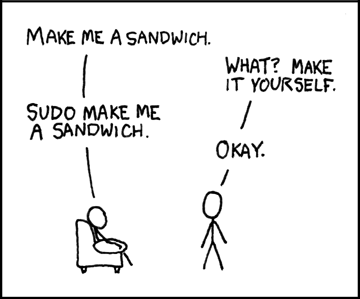
\includegraphics[width=0.95\columnwidth]{res/xkcd/149_sandwich.png}
%	}{\url{https://xkcd.com/149}}
%\end{center}

"Unten" gibt es ein vielfältiges Angebot von immer wiederkehrenden Menüs.
Jeden Tag könnt ihr an der Grillstation Currywurst mit Pommes oder ein Jäger-/Zigeunerschnitzel erwerben.
Montags gibt es den beliebten Mensaburger (auch vegetarisch) in verschiedenen Variationen, welcher so groß ist, dass sich an ihm die Geister scheiden, ob er mit Messer und Gabel oder mit der Hand gegessen werden muss. \textit{[Anm. des Autors: Den Mensaburger ohne Besteck zu essen, ist natürlich einfach falsch!]}
An der Wokstation gibt es häufig Aktionen – meist aber Gerichte, die in großen Pfannen zubereitet werden können. Darunter vermutlich am wichtigsten ist jeden Donnerstag das allseits beliebte (wirklich, die Schlange ist ein Alptraum) Gyros mit Zaziki, viel Krautsalat und Pommes, zu dem durchaus auch Vegetarier greifen, dann aber ohne den Gyrosanteil und mit mehr Kraut.
Dazu gibt es eine Pastatheke, ein Buffet mit Nudeln, Aufläufen und aufgewärmten Resten (häufig eine Anlaufstelle wenn man sonst nichts mag) und ein Salatbuffet, an dem man sich auch Wraps zusammenstellen kann und das sich insbesondere im Sommer großer Beliebtheit erfreut. Allerdings eine Warnung: Die Teller vom Buffet werden an der Kasse nach Gewicht abgerechnet (Das Ganze kostet dann \SI{0,57}{\euro} pro \SI{100}{\g}) und das wird sehr schnell mehr als man beim Zusammenstellen denkt. Außerdem ist ein überquillender Wrap sein eigenes Problem.
Falls ihr Pommes nehmt, ist es empfohlen, mit Pommessalz nachzusalzen und gegen einen kleinen Aufpreis Majo oder Ketchup zu erstehen, Senf ist wie in einer richtigen Frittenbude kostenlos.
Des Weiteren gibt es fast immer einen sehr günstigen Eintopf an der passend genannten Eintopfstation.
Zu jedem Essen gibt es ein recht gutes Angebot an preiswerten Getränken.

Häufig gibt es (meist an der Wokstation) verschiedene Aktionen, so etwa regelmäßig Pizza, deren tatsächlicher Belag nichts mit der Benennung zu tun hat und in der jeweiligen Saison z.\,B. Spargelgerichte oder Erdbeeren mit Schlagsahne. Seit Neuerem bietet die Mensa außerdem regelmäßig Friedensteller an. Dies sind Gerichte, die nach Rezepten der Friedensteller-Intiative (überraschend, ich weiß) gekocht wurden und sich durch Nachhaltigkeit auszeichnen, z.\,B. durch Saisonalität und Regionalität der Zutaten. Diese ersetzen normalerweise eine vegetarische (oder in einigen Fällen vegane) Auswahl "Oben".

Wenn ihr fertig mit dem Essen seid, seid ihr noch lange nicht mit der Mensa fertig!
Entweder ihr holt euch noch einen Nachschlag oder ihr macht euch mit eurem Tablett auf zum Geschirrband und der meist etwas murrig schauenden Person dort.
An der Wand hängt dann eine genaue Anleitung, wie ihr euer Geschirr zu sortieren habt, damit es keinen Ärger vom Mensapersonal gibt.

\fibelimgtext{
	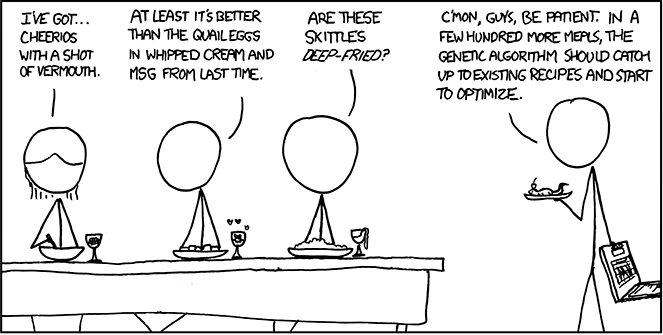
\includegraphics[width=\columnwidth]{res/xkcd/720_recipes.png}
}{\url{https://xkcd.com/720}}

Falls jedoch jemand gar nichts gefunden haben sollte, kann man es auch mit einem Brötchen oder einer Waffel im Café Viva versuchen.
Hier werden auch die meisten anstehenden Sportereignisse übertragen und morgens in der Wiederholung gezeigt.
Außerdem kann man hier recht entspannt sitzen und etwa eine Kaffeespezialität trinken.


Dazu kommen noch diverse Läden wie ein sehr nützlicher Copyshop und Schreibwahrenladen (Kopieren und Drucken ist allerdings preiswerter, wenn man Print~\&~Pay beim ZIV nutzt oder mit dem Guthaben des Studierendenausweis an den Kopierern z.\,B.\ im Lernzentrum, der IG1 oder im ZIV. Aber vergesst eure Karte dort nicht!). Außerdem gibt es noch eine Filiale der Techniker-Krankenkasse und den Aster-Reiseservice.

Alternativ könnt ihr auch die anderen Mensen in Münster besuchen, insbesondere die größte, die Mensa~am~Aasee, sei hier aufgrund der großen Auswahl an Salaten und dem grandiosen Buffet am Abend empfohlen.

\fibelsig{Friedrich, Justus}
\end{multicols*}
